\section{Polarimetric Differential Interferometry}\label{sec:interferometry}


 
%subdiffraction limited, high angular resolution, imaging beyond diff limit, sep
%observable quanitties intrinsically robust against seeing - not directly effected in seeing. Each pair of holes is an interfereomtry - start more general - does a thing thats good, plausible argument that it makes good observables, to understand detail see XY
 

VAMPIRES features a single telescope interferometric mode through use of non-redundant aperture masking (NRM). NRM is implemented with use of an opaque mask perforated by an array of holes in the pupil plane of the instrument (Figure \ref{fig:g18_mask}). The non-redundant spacing of these `sub-apertures' -- wherein each has a unique vector separation -- results in the measurement of unique baseline lengths (Fourier components) of the astrophysical scene \citep{tuthill_aperture_2000}. Unambiguous measurement of each Fourier component yields observables that are robust to atmospheric seeing and to redundancy noise. As a result, NRM allows for the reconstruction of information at angular resolutions at and beyond the diffraction limit (citation).


\begin{figure}[h!]
\centering
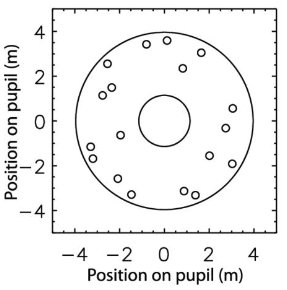
\includegraphics[width=0.7\columnwidth]{figures/g18_mask}
    \caption{\label{fig:g18_mask} g18 mask - copied from \citep{norris_vampires_2015}, to be changed for second draft}
\end{figure}


VAMPIRES combines these advantages of NRM with the aforementioned benefits of polarimetry (\autoref{sec:design}, \autoref{sec:polarimetry}), to achieve sub-diffraction limited measurement of polarized signal within previously inaccessible regions of the image. In particular, the NRM mode unlocks regions that are obscured within the inner-working angle of the coronagraphic mode (\autoref{sec:coronagraphy}). In this way, the NRM and coronagraphic modes operate in a complementary fashion - the outer working angle of the NRM mode is approximately the inner working angle of the coronagraph \citep{norris_vampires_2015}, and together they provide almost complete coverage of the circumstellar environment, right down to the stellar surface. At the cost of some throughput and some Fourier coverage (though minimal for the 18-hole mask), for an appropriate choice of target the NRM mode of VAMPIRES provides exquisite characterization of polarized circumstellar environments, limited only by contrast.


\begin{figure}[h]
\centering
    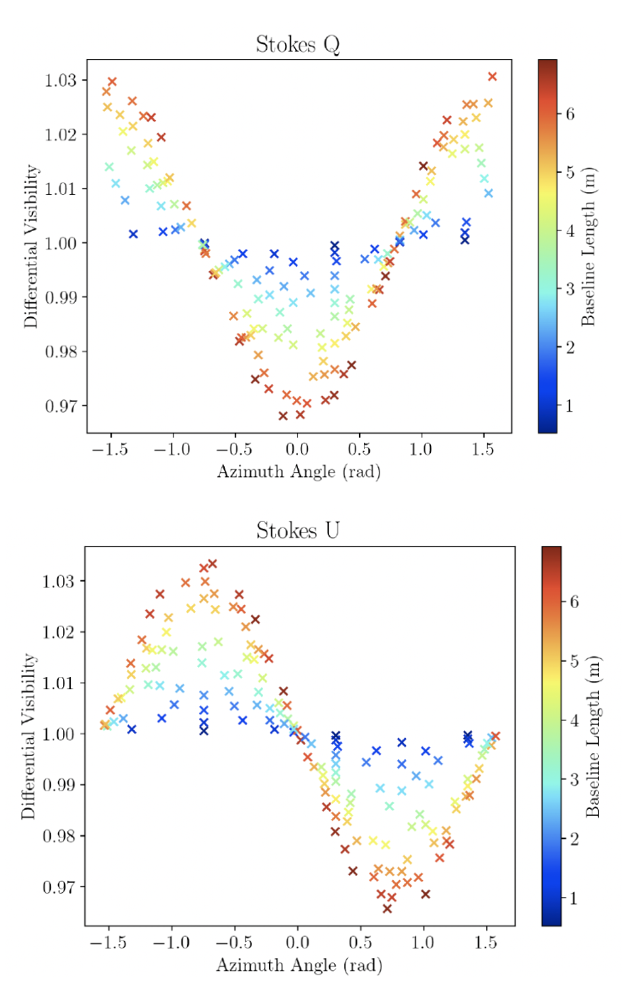
\includegraphics[width=\columnwidth]{figures/diff_vis_all}
    \caption{Polarimetric differential visibilities for model of circumstellar shell. \label{fig:diff_vis_all}}
\end{figure}

The interferometric observables are the differential, polarimetric analogues of standard visibilities and closure phases, and so are self calibrated (no calibrator star is required and errors induced by AO are removed) and relatively immune to non-common instrumental noise \citep{norris_vampires_2015}. We reduce the raw data using the VAMPIRES branch of the AMICAL package (cite, and put at end). Models and images of the astrophysical scene can then be fit to these resulting observables. Techniques for model fitting, as well as novel machine learning based image reconstruction techniques, are currently in development and will be released in the near future, along with early science results obtained using the NRM mode (PI: Lilley, L). 
 
The VAMPIRES upgrade provides several key improvements for NRM. First, the MBI (\autoref{sec:mbi}) mode enables simultaneous measurement of differential observables (eg. spectral differential phase), allowing for the high-precision characterisation of circumstellar dust grain size and species. Not only does this greatly improve observing efficiency compared to repeating observations for different filters, but -- since the time-varying wavefront error is simultaneously sampled across wavelengths -- direct interferometric phase measurements between spectral components can be produced. 
The increased observing efficiency enables the observer to accumulate more parallactic angle coverage, which is critical for characterizing non-azimuthal scattering symmetries. The new qCMOS cameras provide much greater sensitivity than the previous EMCCD cameras, due to their low read noise, which is especially important as the NRM mode requires high frame rates to get high fringe visibility \autoref{sec:detectors}.  
 
We have characterised both the polarimetric calibration precision, as well as the signal to noise for the 4 masks available to the VAMPIRES instrument (Table \ref{tbl:nrm_masks}). The systematic polarimetric calibration limit is 1e-3. Based on polarimetric calibration precision calculations, the sensitivity provided by VAMPIRES is XX. (adapt). This means that a circumstellar disk at contrast 4e-2 around a 5 mag star, assuming a 1 parameter model, would have a 4 sigma detection within 15 minutes. 

%Then quantitative numbers, in terms of both raw visibility or closure phase precision for a given stellar mag / integration time, and the polarised-differential-visibilty calibration accuracy.
 
\begin{deluxetable*}{lccccc}
% TODO - mask throughput, SNR for 0 mag 1s (or similar), time to achieve desired precision (10^-3 error) for typical star mag
\tablehead{\colhead{Name} & \colhead{N Holes} & \colhead{Hole Radius (m)} & \colhead{Num Baselines} & \colhead{Throughput (\%)} & \colhead{S/N} }
\tablecaption{VAMPIRES NRM mask specifications.\label{tbl:nrm_masks}}
\startdata
SAM-18 & 18 & 0.162  & 153 & 0.74 & 3400\\
SAM-9 & 9 & 0.32       &  36   & 1.4 & 18750\\
SAM-7 & 7 & 0.55&   28        & 3.1 & 83000 \\
SAM-Ann & 4 &   &              & & \\
\enddata
\tablecomments{S/N is calculated for 10 ms exposures, 100 frames (1 second total integration time), for a 0 mag star}
\end{deluxetable*} 
\vspace{3mm}
 
  



%are obscured by the inner-working angle of the coronagraph


%Unlike the coronagraphic mode (cite section), there is no strict inner-working angle to the NRM mode - rather, the NRM mode has an outer working angle dictated by its shortest baseline length, and is limited within this field only by contrast. By design (?) 

%, for example, innermost circumstellar environments. VAMPIRES is able to probe these regions at scales of down to 10 mas, at arbitrarily close distances from the stellar surface. The observation of inner circumstellar envelopes is crucial for understanding the physics of evolved star mass loss, which characterises the end stage of life of evolved stars, yet remains an incompletely understood phenomena (reference).





%Calibration precision etc. With enough light - precision / measurement. Diff vis cal in 1/10e3, sd is 10e-3 with no noise, 1 parameter, normally distributed noise, 100 baslines, 1 degree of freedom, measure total parameter in 1/10e4. what does it correspond . Disks, decrease contrasts, when mag of wiggle is same as sd of measurement - 1 sigma measurement. variance of signal == variance of noise. when is sd of signal comparable with sd of systematics. 1 sigma detection. Sd of visibilities vs sd of noise. When is SNR 1. Fit model with 1 parameter - scale that. Perfect disk of contrast of 10e-4 would be a 1 sigma detection.

 

%, and is responsible for some of the highest resolution %images in modern astronomy (reference). 
 




 
 %The target is required to be appropriate for NRM - it must have sufficient brightness and its angular extent must be comparable with the longest NRM mask baseline length to ensure there is sufficient coherence for observable interference.

 
 
%The mask generates an interference pattern on the detector, the contrast of the interference fringes has a mathematical relationship to the underlying source distribution and can to reconstruct images \citep{labeyrie_introduction_2014}. 
 

%The more sub-apertures, the better the Fourier coverage, but the less photons or throughput (this comes as a consequence of requiring smaller holes as more are added, to maintain signal to noise in Fourier space).
